% TEX compiler = luatex
% copyright arturo salinas-aguayo 2025
\documentclass[12pt]{article}

\usepackage{graphicx}
\usepackage{amsmath}
\usepackage{array}
\usepackage{amsfonts}
\usepackage{fancyhdr}
\usepackage{geometry}
\usepackage{circuitikz}
\usepackage{subfigure}
\usepackage{caption}
\usepackage{karnaugh-map}
\usepackage{bm}
\usepackage{float}

\geometry{letterpaper, margin=1in}
\graphicspath{ {../../images/} }

% Header and Footer
\pagestyle{fancy}
\fancyhf{}
\fancyhead[L]{ECE 2001 - Lab 03: Op Amps, Comparators, and Resistive Sensors}
\fancyhead[R]{\thepage}
\setlength{\headheight}{15pt}

\author{Arturo Salinas-Aguayo}
\title{Lab 03: Op Amps, Comparators, and Resistive Sensors}
% theorem set
\newtheorem{example}{Example}
% Example block environment
\newenvironment{examp}
{\vspace{0.5cm}
 \hrule
\vspace{0.5cm}
\begin{example}}
{\hrule
\vspace{0.5cm}
\end{example}}

\begin{document}
\newcommand{\closure}[2][3]{%
	{}\mkern#1mu\overline{\mkern-#1mu#2}}
\newcommand\ncoverline[1]{\mkern1mu\overline{\mkern-1mu#1\mkern-1mu}\mkern1mu}
% Title Page
\begin{titlepage}
	\centering
	\vspace*{3cm}
	\huge\textbf{Lab 03: Op Amps, Comparators, and Resistive Sensors}\\
	\vspace{5cm}
	\Large\textbf{Arturo Salinas-Aguayo}\\
	\normalsize
	ECE 2001 Electrical Circuits\\
	Dr. David J. Giblin, Section 331.660.701.810-1253\\
	Mechanical Engineering Department
	\vfill
	
\includegraphics[scale=0.1]{uconnlogo}\\
	College of Engineering, University of Connecticut\\
	\scriptsize{Coded in \LaTeX}
	\vspace*{1cm}
\end{titlepage}
\tableofcontents
\newpage
\section{Abstract}
This experiment aims to teach the basic properties of operational amplifies (Op
Amps). Through the use of the ADALM2000 and several different circuits, the Op
Amp's properties are explored. By creating a single comparator circuit and an
amplifier circuit, the linear region of the op amp is exploited and put on show.
By starting out with no feedback, it is made apparent to how quickly
the op amp saturates and how impractical its use in a system like this would be.
After applying a feedback loop to the circuit through the use of potentiometers
(pots) and a photoresistor, the operational use of the op amp is demonstrated in
a physical manner. A small simulation in production ready simulation tools is
also included to further stimulate the knowledge on op amps.
\newpage
\section{Introduction}
The operational amplifier is a component which can serve many applications,
including operating as a differentiator or integrator, as well as other
mathematical operations. This provides an analog to the ALU that was taught in
CSE2301, in which a digital logic circuit provided a means to shift and
manipulate bits stored in registers. The operational amplifier however, is an
analog tool that predates the modern sense of an ALU, yet is a powerful tool to
understand how certain things such as impedance, amplification gain, and
operational characteristics can impact a circuit and its design.

The operational amplifier was introduced in 1947 by John Ragazzini at the
National Defense Research Council after World War II. This aligns with the start
of the cold war, a time of exponential technological growth, similar to the
component itself. This weeks lessons on the operational amplifier abstracted away the inner
workings in a ``black box" approach to studying the component. This allowed for
the abstract analysis of several circuits such as an inverting amplifier, a
non-inverting amplifier, a summing circuit, and a subtracting circuit, called
the  difference amplifier.

In essence, further elaborated upon in the proceeding sections, the component
acts as a voltage amplifier with a dedicated power supply with a very high gain.
When considered \textit{ideal}, there are certain assumptions that can be made
about the component which allows for the extensive analysis of circuits that it
is embedded into.

This Op Amp, when combined with other tools such as potentiometers and
photoresistors allow for the use of some unique circuits such as the ones built
for this experiment.

\section{Theory}

\subsection{The Operational Amplifier}
The Operational Amplifier (Op Amp) is an electrical component that allows for an
abstracted sense of mathematical operations within a circuit. Functions such as
addition, subtraction, multiplication, division, and even calculus such as
differentiation and integration are all possible with the correct use of this
component.

It is made up of an assortment of resistors, transistors, capacitors, and
diodes, however this experiment abstracts most of that away with the
aforementioned ``black box" approach. That is to say, the inner workings of the
component itself are not delved into in particular. The DIP (Dual-In-Line)
package used is the \(\mu A 741\) chip shown in Figure \ref{741}.
\begin{figure}[H]
	\centering
	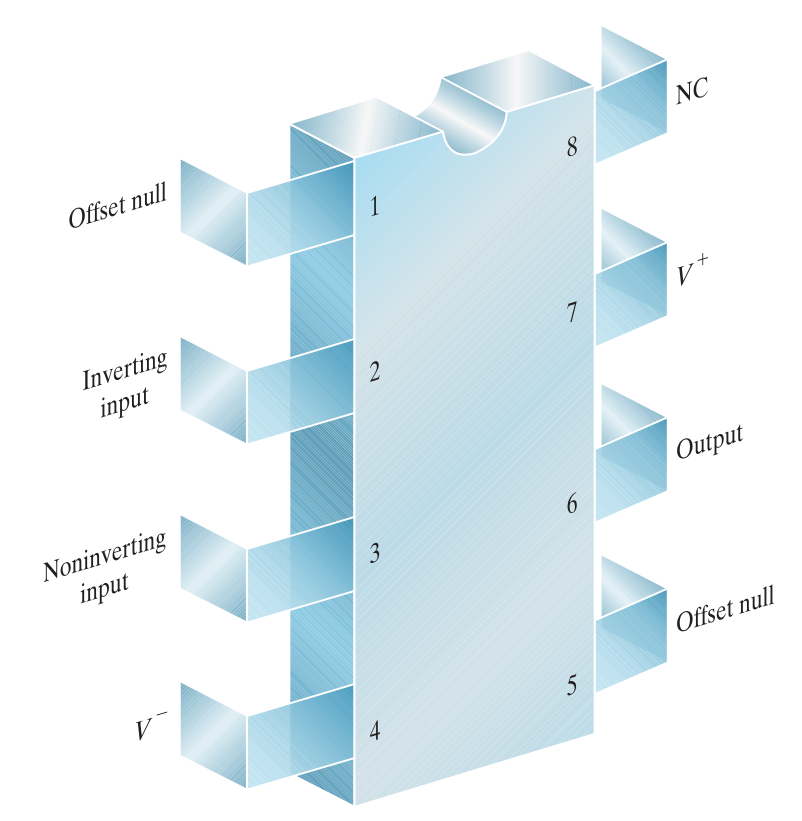
\includegraphics[width=8cm]{02_1}
	\caption{The \(\mu A 741\) }
	\label{741}
\end{figure}
The basic equation for the Op Amp has a lot to do with its specific gain, \(A\).
where:
\[
	V_{out} = A(\upsilon_p - \upsilon_n)
\]
For a specific region called the \textit{linearly operational region}

\subsection{Linear Operation of Terminal Voltages}
The Operational Amplifier quickly saturates in certain cases, which is not a
desirable outcome in most applications. Quickly if the input voltage at either
of the terminals (\(\upsilon_p\) for the positive terminal and \(\upsilon_n\)
for the negative terminal)  reaches beyond the supplied \(V_{cc}\), the output
voltage is pegged, or \textit{saturated}. This is similar to maxing out a car
stereo where it gets so loud that the output is just \textit{noise}.

It is up to the circuit designer to consider this effect and build the circuit
so it can operate in the linear region. When in the linear region,
\[
	\upsilon_n = \upsilon_p
\]
For an ideal op amp with an infinite gain.

This constraint, however can only be taken advantage of in the aforementioned
linear operation region. The other constraint, however, has to do with the
infinite gain mentioned earlier.

For an ideal op amp, the impedance felt at the positive and negative terminals
is infinite, which means that for calculations, one can \textit{always assume}:
\[
	i_p = i_n = 0
\]
This means that the current flowing into the opamp at its terminals is
effectively null and can vastly simplify calculations.

\subsection{The Potentiometer}
A potentiometer is a three-terminal variable resistor that allows for the
adjustment of resistance via a mechanical control, typically a rotating knob or
a sliding mechanism. The potentiometer used in this experiment is a \(10k\Omega\)
linear potentiometer rated at 0.25W. This component
enables precise control of voltage within a circuit by acting as a voltage
divider or a rheostat, depending on the circuit configuration.

In the voltage divider configuration, the potentiometer is connected such that the wiper moves along the resistive element, dividing the input voltage (\(V_{in}\)) into two output voltages, one of which varies according to the wiper position:
\[
	V_{out} = V_{in} \times \frac{R_2}{R_1 + R_2}
\]
where \( R_1 \) and \( R_2 \) are the resistances formed by the wiper's position
along the resistive track. When used as a variable resistor (rheostat), one
terminal is left unconnected, and the resistance between the wiper and one fixed
terminal varies from nearly zero to the maximum rated resistance (\(10k\Omega\) in this case).

The linear characteristic of the selected potentiometer means that the resistance change is directly proportional to the wiper’s displacement. This ensures a predictable and uniform change in resistance, which is useful for applications such as tuning, signal attenuation, and sensor calibration. The power rating of 0.25W ensures it can handle moderate electrical loads without excessive heat dissipation.

When integrating the potentiometer into the circuit, considerations such as contact resistance, mechanical durability, and wiper noise should be taken into account, particularly in precision applications where fluctuations in resistance could impact system performance.

\subsection{The Photoresistor}
A photoresistor, or light-dependent resistor (LDR), is a variable resistor whose
resistance changes as a function of incident light intensity. The Luna
Optoelectronics PDV-P8001 photoresistor used in this experiment has a resistance
range of \(3k\Omega\) to \(11k\Omega\) and a diameter of 5.10mm. This component is particularly
useful in circuits requiring light sensitivity, such as automatic lighting
controls and optical detection systems.

The fundamental working principle of a photoresistor is based on photoconductivity, where increased light intensity reduces the material’s resistivity due to photon-induced excitation of charge carriers. The relationship between incident light intensity (\(E\)) and resistance (\(R\)) can be approximated by:
\[
	R = R_d \times E^{-\gamma}
\]
where \(R_d\) is the dark resistance (resistance in complete darkness), and \(\gamma\) is a material-dependent constant that typically ranges between 0.7 and 0.9 for cadmium sulfide (CdS) photoresistors.

When incorporated into a voltage divider circuit, the photoresistor can be used to generate a variable voltage output corresponding to changes in ambient light levels:
\[
	V_{out} = V_{cc} \times \frac{R_{LDR}}{R_{LDR} + R_{fixed}}
\]
where \(R_{LDR}\) is the resistance of the photoresistor and \(R_{fixed}\) is a reference resistor. This configuration enables the conversion of light intensity variations into a measurable electrical signal, which can then be processed by microcontrollers or analog circuits for automation and feedback control.

Practical considerations for implementing the PDV-P8001 include its spectral response, response time, and temperature sensitivity. The response time of the photoresistor varies with light intensity changes, typically in the range of milliseconds to seconds, making it suitable for slow-to-moderate response applications but less ideal for high-speed optical sensing. Additionally, variations in ambient temperature can affect the resistance characteristics, requiring compensation in precision applications.

By incorporating both the potentiometer and photoresistor in the circuit, a dynamic and adaptable voltage control system can be achieved, useful in applications such as dimming controls, sensor calibration, and interactive electronic designs.

\section{Experimental Procedures}

\subsection{A Quickly Saturated Beginning}
The first experiment utilized the circuit shown in Figure \ref{fig:first}


\begin{figure}[H]
	\centering
	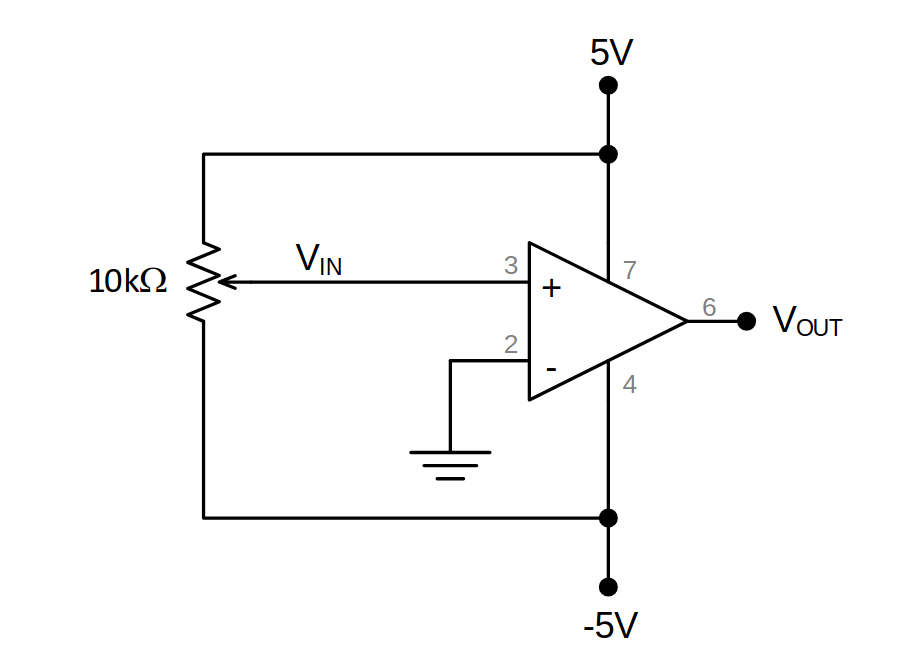
\includegraphics[width=8cm]{02_2}
	\caption{A Feedbackless Op Amp}
	\label{fig:first}
\end{figure}

\begin{enumerate}
	\item This circuit is called a \textit{Non-Inverting Amplifier Circuit}

	      It is a peculiar construction as since there is no feedback loop from
	      \(V_{out}\) back to the input at \(\upsilon_p\) it quickly saturates as
	      the potentiometer is modified

	\item The voltage at the \(\upsilon_p\) terminal was recorded via Scopy
	      software through the ADALM2000.

	      The output voltage at \(V_{out}\) was
	      monitored via multimeter.

	\item The output voltage, \(V_{out}\), was measured at small intervals after modifying the
	      potentiometer wiper position

	      Table \ref{tab:measured_data} contains the data recorded for this first
	      portion. Notice that the circuit quickly saturates with almost no
	      ability to finely be able to tune the voltage to the linear region. This
	      is expected.
\end{enumerate}
\subsection{Comparing Two Input Voltages}
The second experiment utilized the circuit shown in Figure \ref{fig:comparator}

\begin{figure}[H]
	\centering
	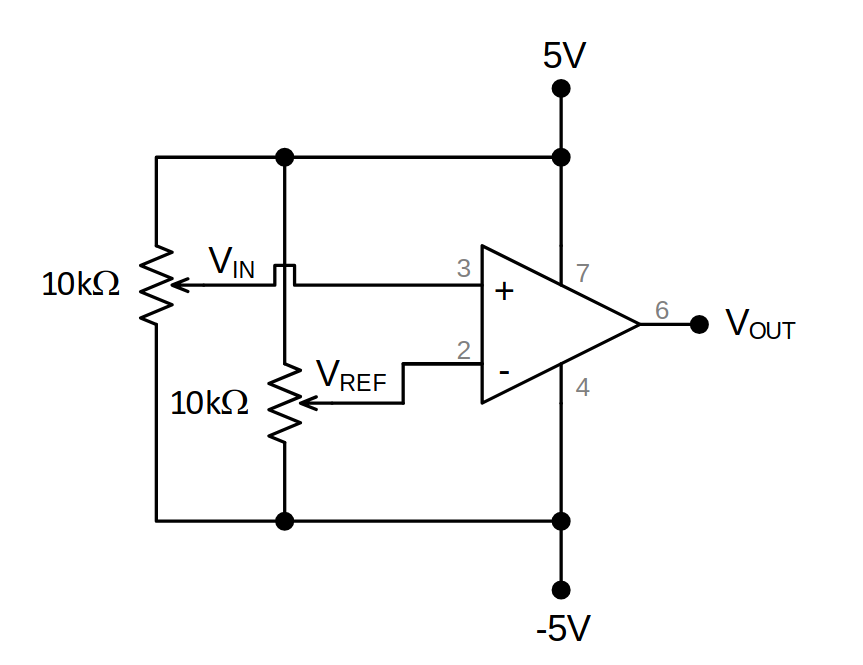
\includegraphics[width=8cm]{02_3}
	\caption{A Basic, Feedbackless Comparator}
	\label{fig:comparator}
\end{figure}
\begin{enumerate}
	\item This circuit is called a \textit{Comparator} which compares the two
	      inputs into the operational amplifier.
	\item The difference here is that the reference voltage, or \(V_{ref}\)
	      allowed for a granularity in the opposite input terminal,
	      \(\upsilon_n\).

	      Unfortunately, since the circuit still has no feedback, it very quickly
	      saturated to \(V_{CC}\) and \(V_{EE}\)

	\item The output voltage, \(V_{out}\), was measured at small intervals after modifying the
	      potentiometer wiper position. One set of data was recorded with the
	      reference potentiometer at a minimum wiper position, while another was
	      set at maximum. Educationally, this allowed for a change in the output
	      voltages as the circuit attempted to hold true to its characteristics.

	      Table \ref{tab:comparator} contains the data recorded for this first
	      portion.
\end{enumerate}

\subsection{A Mini-Design Challenge}
This portion of the experiment provided the freedom to design a circuit which is
responsive to the natural world. I chose to employ the photoresistor as a bridge
to the negative terminal in order to accomplish the task of having an LED shine
brightly as the resistance in the photoresistor increased, that is, got darker.

The desired characteristics were displayed and a circuit design that looks like
Figure \ref{fig:photoresistor} was incorporated.

\begin{figure}[H]
	\centering
	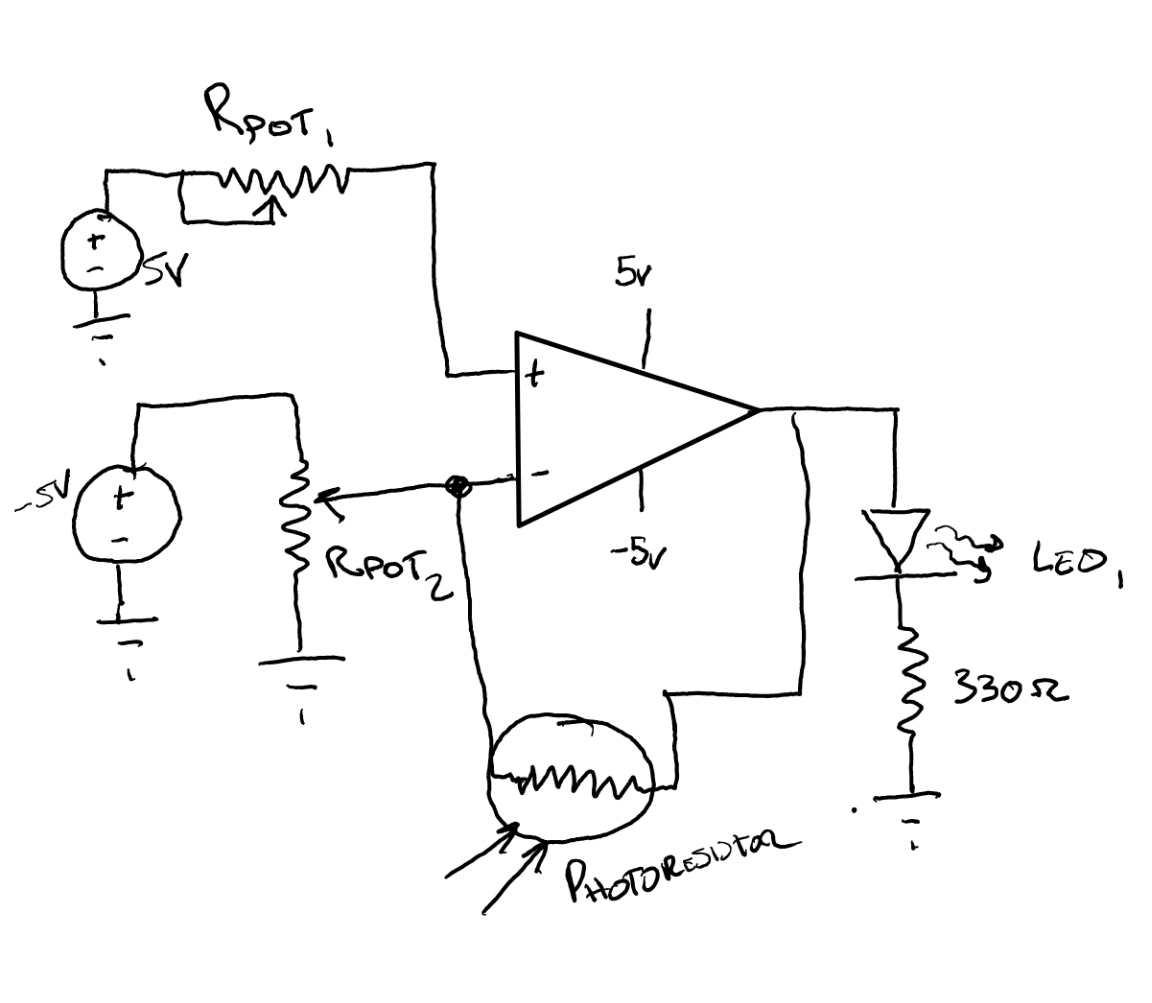
\includegraphics[width=8cm]{02_4}
	\caption{First Design, Photoresistor in Feedback}
	\label{fig:photoresistor}
\end{figure}

\begin{enumerate}
	\item Resistance cannot be measured with the component energized. It will not
	      be accurate due to how an ohmmeter relies on it's supplied current to get an
	      accurate measure of resistivity.

	      The Photoresistor's characteristics were measured at full dark, and full
	      light with a cell phone flashlight to simulate full bright conditions.
	\item \(V_{out}\) was measured at various conditions. This was experimentally
	      problematic as there is no sure fire way in our setup to get a certain
	      percentage of light. Nevertheless various voltages were recorded and notated
	      in Table \ref{tab:photoresistor}.
\end{enumerate}

\subsection{An Inverting Amplifier with Feedback}
The fourth experiment utilized the circuit shown in Figure \ref{fig:inverter}

\begin{figure}[H]
	\centering
	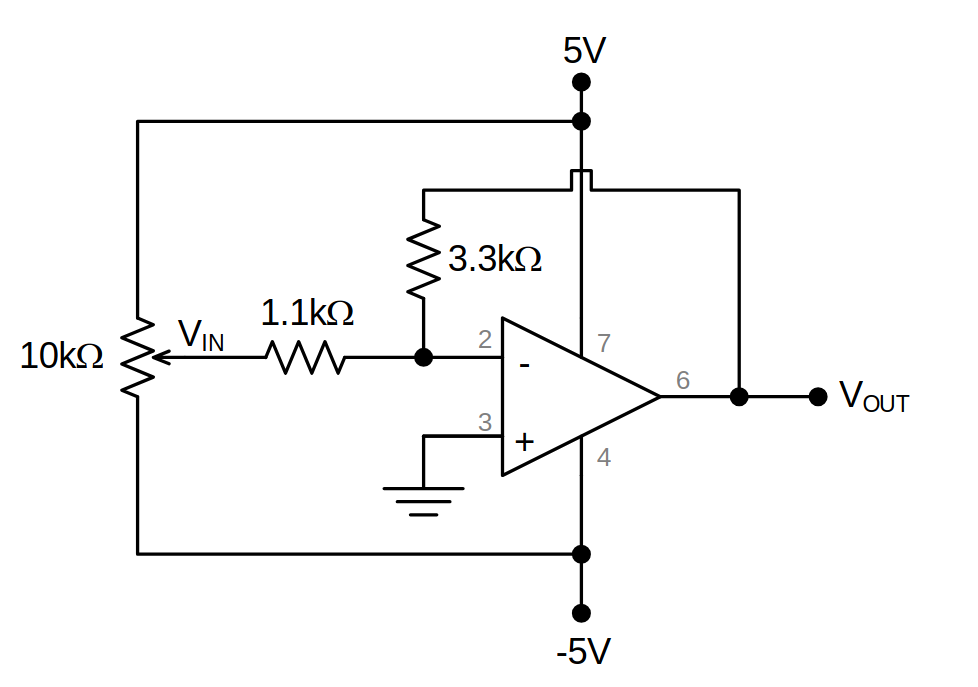
\includegraphics[width=8cm]{02_5}
	\caption{An Inverting Amplifier with Feedback}
	\label{fig:inverter}
\end{figure}

\begin{enumerate}
	\item An inverting amplifier was configured to emphasize now how the linear
	      region operates.
	\item Positive and negative values of \(V_{in}\) provided a different
	      operating characteristic under these conditions.
	\item Output results are populated in Figure \ref{fig:03_pspice}
\end{enumerate}

\subsection{Allegro Cadence PSpice Segue}
The last part of the experimentation compared the built circuit in the previous
part to a simulated circuit utilizing Allegro Cadence PSpice simulation. The
circuit built is provided in Figure \ref{fig:pspicecircuit}


\begin{figure}[H]
	\centering
	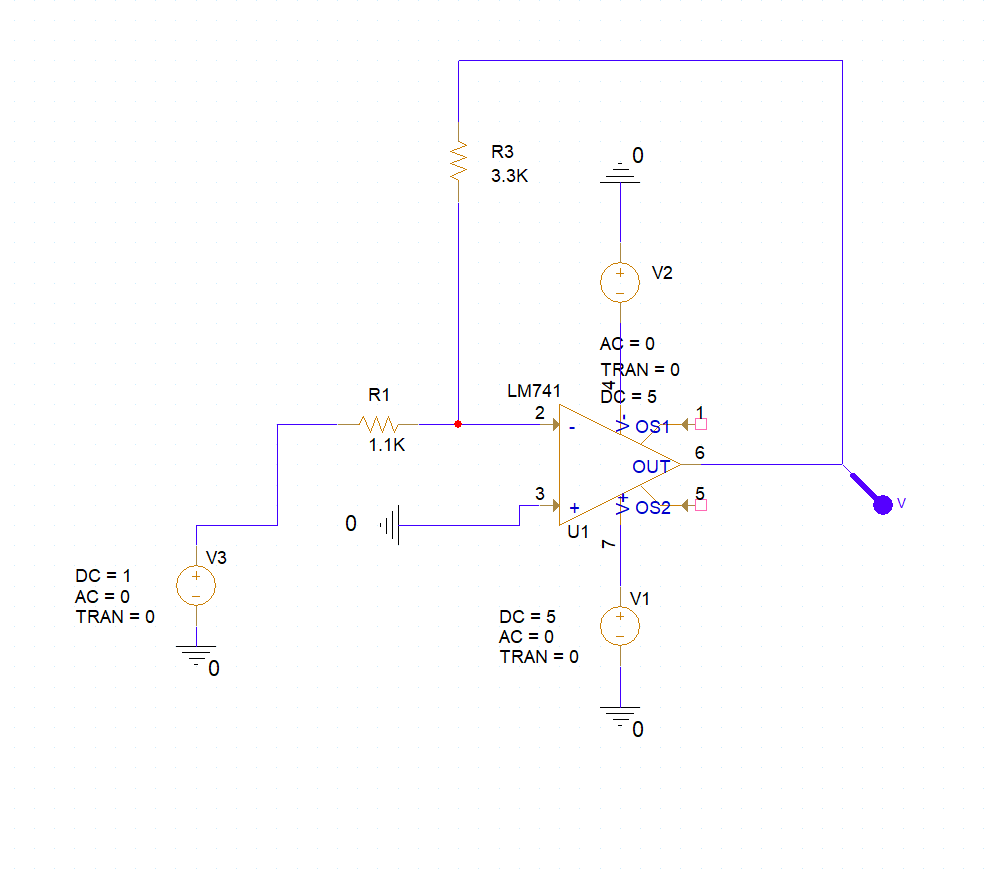
\includegraphics[width=12cm]{03_7}
	\caption{Cadence Simulated Circuit}
	\label{fig:pspicecircuit}
\end{figure}
\begin{enumerate}
	\item The circuit was built in the simulator utilizing parts that closely
	      resembled the real hardware used previously.
	\item Instead of a potentiometer sweep, a DC Voltage sweep was conducted for
	      ease of use and plotting from -5V to 5V.
	\item This was able to get down the the microvolts the linear region that
	      was not able to be seen in data closely using the potentiometer sweep.
	\item Preliminary data seen from the simulator in Figure
	      \ref{fig:pspicesweep}

	      \begin{figure}[H]
		      \centering
		      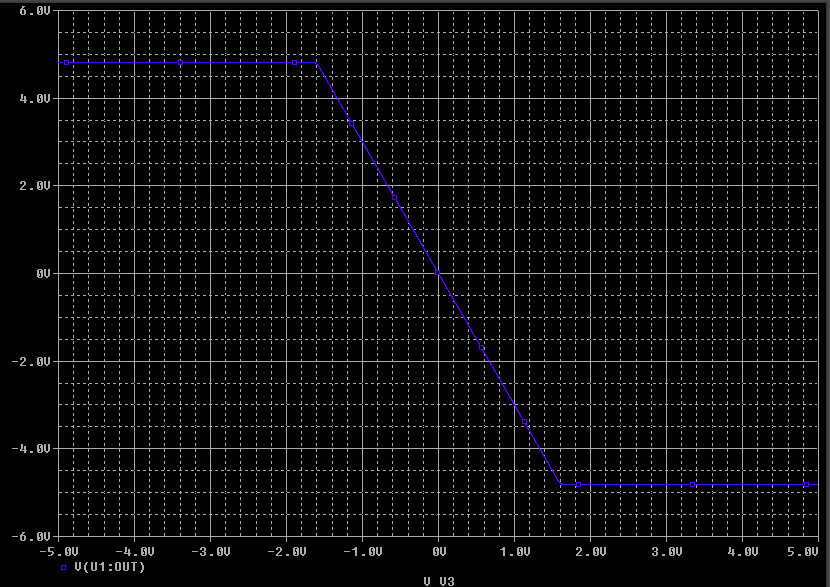
\includegraphics[width=12cm]{03_6}
		      \caption{PSpice Sweep}
		      \label{fig:pspicesweep}
	      \end{figure}
\end{enumerate}

\section{Results and Discussion}
\subsection{A Quickly Saturated Beginning}

The first experiment demonstrated how an operational amplifier without feedback rapidly saturates. As seen in Table \ref{tab:measured_data}, even small changes in input voltage resulted in immediate saturation to either the positive or negative supply rails. This behavior is expected since, in the absence of feedback, the operational amplifier functions as an open-loop amplifier with an exceedingly high gain. This high gain causes even minute input voltage variations to push the output to its limits.

Figure \ref{fig:exp1} visually represents this saturation effect. The practical
implication of such a circuit is that it cannot be used for controlled
amplification but is rather suited for comparator applications. High Saturation
and low saturation voltages are plotted in Figure \ref{fig:exp1}.
\begin{table}[H]
	\centering
	\begin{tabular}{|c|c|}
		\hline
		$V_{in}$ (V) & $V_{out}$ (V) \\
		\hline
		4.961        & 4.44          \\
		4.226        & 4.44          \\
		3.742        & 4.44          \\
		3.124        & 4.45          \\
		2.756        & 4.45          \\
		2.065        & 4.45          \\
		1.641        & 4.45          \\
		1.027        & 4.45          \\
		0.565        & 4.45          \\
		0.048        & 4.45          \\
		-0.043       & -3.00         \\
		-0.168       & -3.03         \\
		-0.314       & -3.09         \\
		-1.582       & -3.04         \\
		-2.382       & -3.04         \\
		-3.408       & -3.04         \\
		-5.078       & -3.04         \\
		\hline
	\end{tabular}
	\caption{Measured Input and Output Voltages}
	\label{tab:measured_data}
\end{table}


\begin{figure}[H]
	\centering
	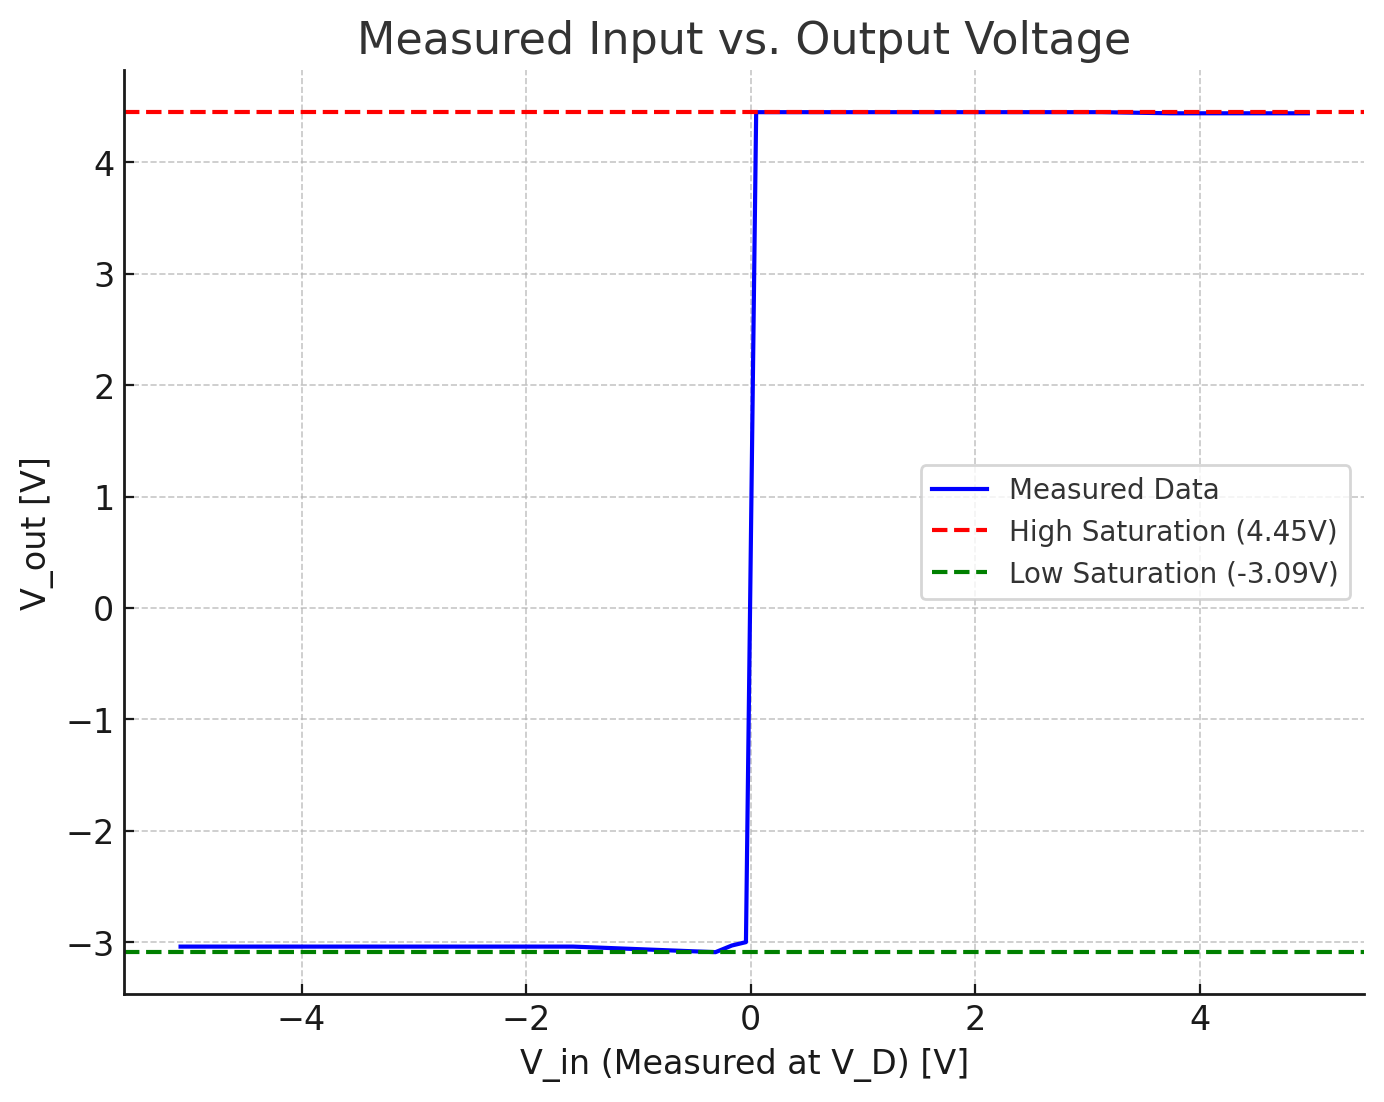
\includegraphics[width=12cm]{03_exp1}
	\caption{A Quickly Saturated Amplifier}
	\label{fig:exp1}
\end{figure}

\subsection{A Comparator Circuit, Modulating Reference Voltage}
Introducing a reference voltage, $V_{REF}$, provided a method to compare the input voltage against a defined threshold. The experimental data in Table \ref{tab:comparator} reveal that changing the reference voltage alters the transition point at which the amplifier output flips between the supply rails.

As illustrated in Figure \ref{fig:exp2}, the comparator circuit continues to
exhibit the characteristic rapid switching between extremes, confirming that it
is well-suited for binary decision-making applications. However, the inability
to finely control the output voltage without saturation still poses challenges
when precise analog outputs are required. The data points show that the
comparator simply outputs the saturation voltage of the greater of the two
potentials.
\begin{table}[H]
	\centering
	\caption{Measured Data for Different $V_{REF}$ Settings}
	\begin{tabular}{|c|c|}
		\hline
		$V_{in}$ (V) & $V_{out}$ (V)                                               \\
		\hline
		\multicolumn{2}{|c|}{\textbf{$V_{REF}$ More Negative ($R_{pot2}$ at Min)}} \\
		\hline
		5.028        & -2.881                                                      \\
		3.775        & -3.04                                                       \\
		2.973        & -3.04                                                       \\
		-1.330       & -3.04                                                       \\
		-2.666       & -3.04                                                       \\
		-3.541       & -3.04                                                       \\
		-4.193       & -3.04                                                       \\
		-4.894       & -3.04                                                       \\
		-5.078       & -3.04                                                       \\
		\hline
		\multicolumn{2}{|c|}{\textbf{$V_{REF}$ More Positive ($R_{pot2}$ at Max)}} \\
		\hline
		4.961        & 4.45                                                        \\
		3.391        & 4.45                                                        \\
		2.382        & 4.45                                                        \\
		1.828        & 4.45                                                        \\
		0.824        & 4.45                                                        \\
		-0.592       & 4.45                                                        \\
		-1.606       & 4.45                                                        \\
		-3.458       & 4.45                                                        \\
		-4.727       & 4.45                                                        \\
		-5.078       & 4.45                                                        \\
		\hline
	\end{tabular}
	\label{tab:comparator}
\end{table}

\begin{figure}[H]
	\centering
	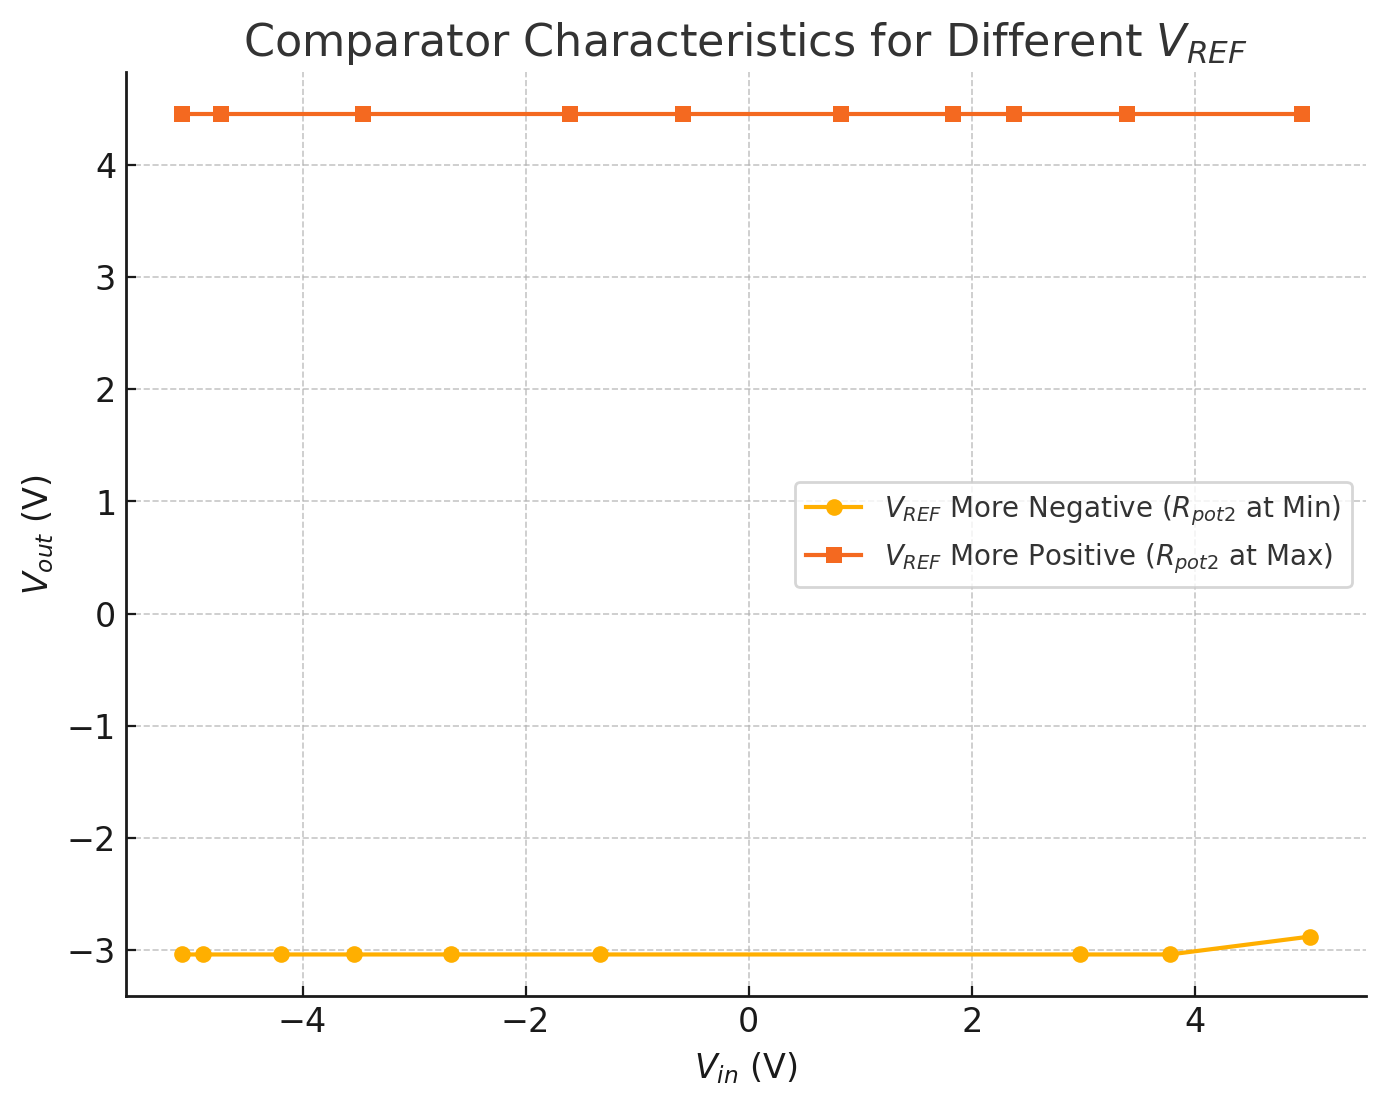
\includegraphics[width=12cm]{03_exp2}
	\caption{Comparator Circuit Characteristics}
	\label{fig:exp2}
\end{figure}

It is displayed quite obviously that the feedbackless operational amplifier
chooses to saturate based on input conditions alone. Either the output voltage
was positive saturation or negative saturation, nothing else, yet the values
felt at the output were slightly changed than the first part due to the circuit
design.

\subsection{An Automatic Night Light Circuit}
The experiment involving the photoresistor-based automatic night light circuit
successfully showcased the behavior of the component under varying light
conditions. The measured resistance values at full light (0.197 k$\Omega$) and
full darkness (14.92 k$\Omega$) highlight the significant resistance change as
light intensity varies.

Table \ref{tab:photoresistor} demonstrates the corresponding output voltages,
showing a clear inverse relationship between light intensity and output voltage.
As expected, the LED brightness increased in darkness due to the decreasing
feedback resistance, leading to a higher output voltage.

The fitted curve in Figure \ref{fig:exp3} validates the nonlinear nature of the
photoresistor response, showing a logarithmic trend rather than a linear
progression. This confirms the expected exponential change in resistance as a
function of illumination intensity, an essential characteristic for night-light
circuit designs.

\begin{table}[H]
	\centering
	\begin{tabular}{|c|c|}
		\hline
		\textbf{Light Condition}     & \textbf{Voltage ($V_{out}$)} \\
		\hline
		Full Light (0.197 k$\Omega$) & 0.334 V                      \\
		\hline
		1/3 Dark                     & 1.725 V                      \\
		\hline
		2/3 Dark                     & 2.15 V                       \\
		\hline
		7/9 Dark                     & 2.63 V                       \\
		\hline
		Full Dark (14.92 k$\Omega$)  & 3.60 V                       \\
		\hline
	\end{tabular}
	\caption{Photoresistor Node Voltages under Different Light Conditions}
	\label{tab:photoresistor}
\end{table}


\begin{figure}[H]
	\centering
	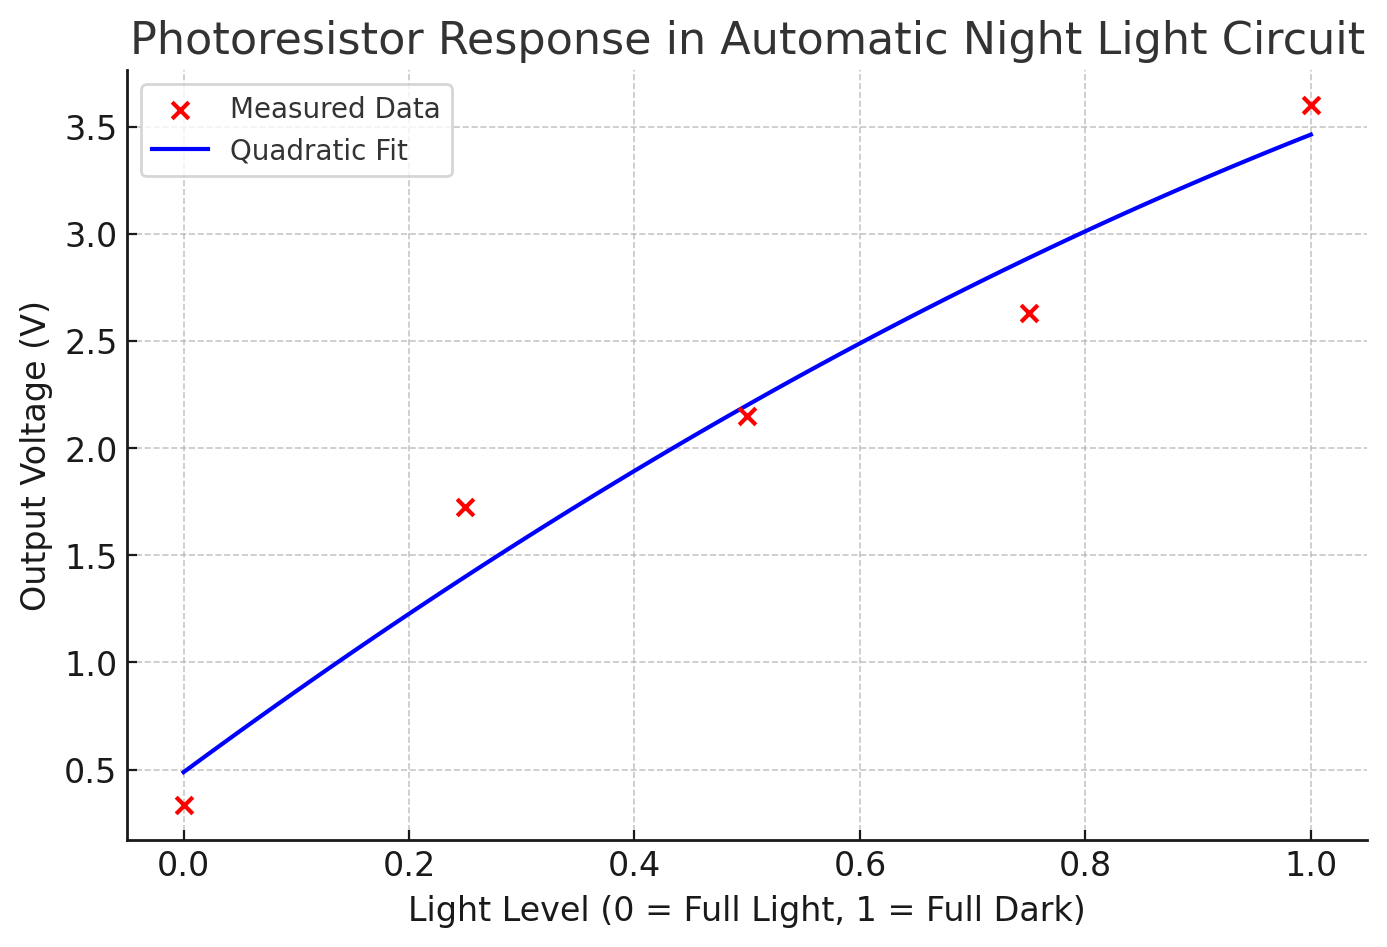
\includegraphics[width=12cm]{03_exp3}
	\caption{Night Light Circuit Characteristics}
	\label{fig:exp3}
\end{figure}

The design choice of using the photoresistor as an inverting feedback resistor
was made deliberately in order to give better linearity to the behavior of the
circuit. This was perhaps different than the task to simply use it as an input
resistance, but in effect this circuit is superior and adheres to better
practices in the use of operational amplifiers by widening the linear response
region while still solving the design problem.
\subsection{An Inverting Op-Amp}
Unlike the previous circuits, the inverting amplifier configuration in Figure \ref{fig:inverter} utilized feedback to establish a stable linear region of operation. Table \ref{tab:inverting_amp} presents measured data that confirm the expected inverting gain relationship between $V_{in}$ and $V_{out}$.

Unlike previous circuits, this setup allowed for a controlled output range, as
seen in Table \ref{tab:inverting_amp}. The amplifier effectively operated within
its linear range before hitting saturation limits, demonstrating a stark
contrast to the open-loop configurations tested earlier. The use of this circuit
is much more apparent now with negative feedback. It amplifies the voltage felt
at the negative terminal by a factor which is proportional to the feedback
resistor and the input resistance.

During experimentation, there was a ``deadzone" in the potentiometer position
and the input voltage to the circuit which lasted from \(-0.060V \implies
+0.060V\). This made obtaining data difficult in this region, but it is expected
behavior! As when in the linear region, the operational amplifier applies
something called a voltage short condition where the potential felt at the
terminals are equal to each other. This allowed for granularity in the output
which show a clear linear relationship as the potentiometer was positioned.

This is later confirmed in the Cadence PSpice simulator to be on the scale of
nanovolts, which was quite interesting.
\begin{table}[H]
	\centering
	\begin{tabular}{|c|c|}
		\hline
		$V_{in}$ (V) & $V_{out}$ (V) \\
		\hline
		2.940        & -2.85         \\
		1.852        & -2.87         \\
		1.359        & -2.88         \\
		0.920        & -2.89         \\
		0.346        & -2.90         \\
		-0.006       & 3.97          \\
		-0.605       & 4.19          \\
		-1.154       & 4.19          \\
		-2.014       & 4.17          \\
		-2.723       & 4.16          \\
		\hline
	\end{tabular}
	\caption{Measured Data for Inverting Amplifier Circuit}
	\label{tab:inverting_amp}
\end{table}
This data shows a linear region in which output voltages were linearly swept
through while the voltage felt at the negative inverting terminal was kept
shorted to the positive terminal by the voltage short characteristic. As soon as
the operational amplifier reached saturation, voltages at the negative terminal
were able to be recorded as in the previous examples. These outcomes and
behavior was expected.

\subsection{The Ideal Simulated Case}
The final experiment compared measured results to those obtained from PSpice
simulations. This matches up with the behavior seen in the lab, although at
slightly different voltages due to tolerances in the experiment. This is
expected behavior.

The PSpice-generated curve in Figure \ref{fig:03_pspice} illustrates the precise
theoretical behavior of the circuit. When zoomed in on, it exhibits expected
behavior at a much smaller scale that could be measured in the lab experiment,
although it was behaviorally showed in the output voltages. See previous Figure
\ref{fig:pspicesweep}.

\begin{figure}[H]
	\centering
	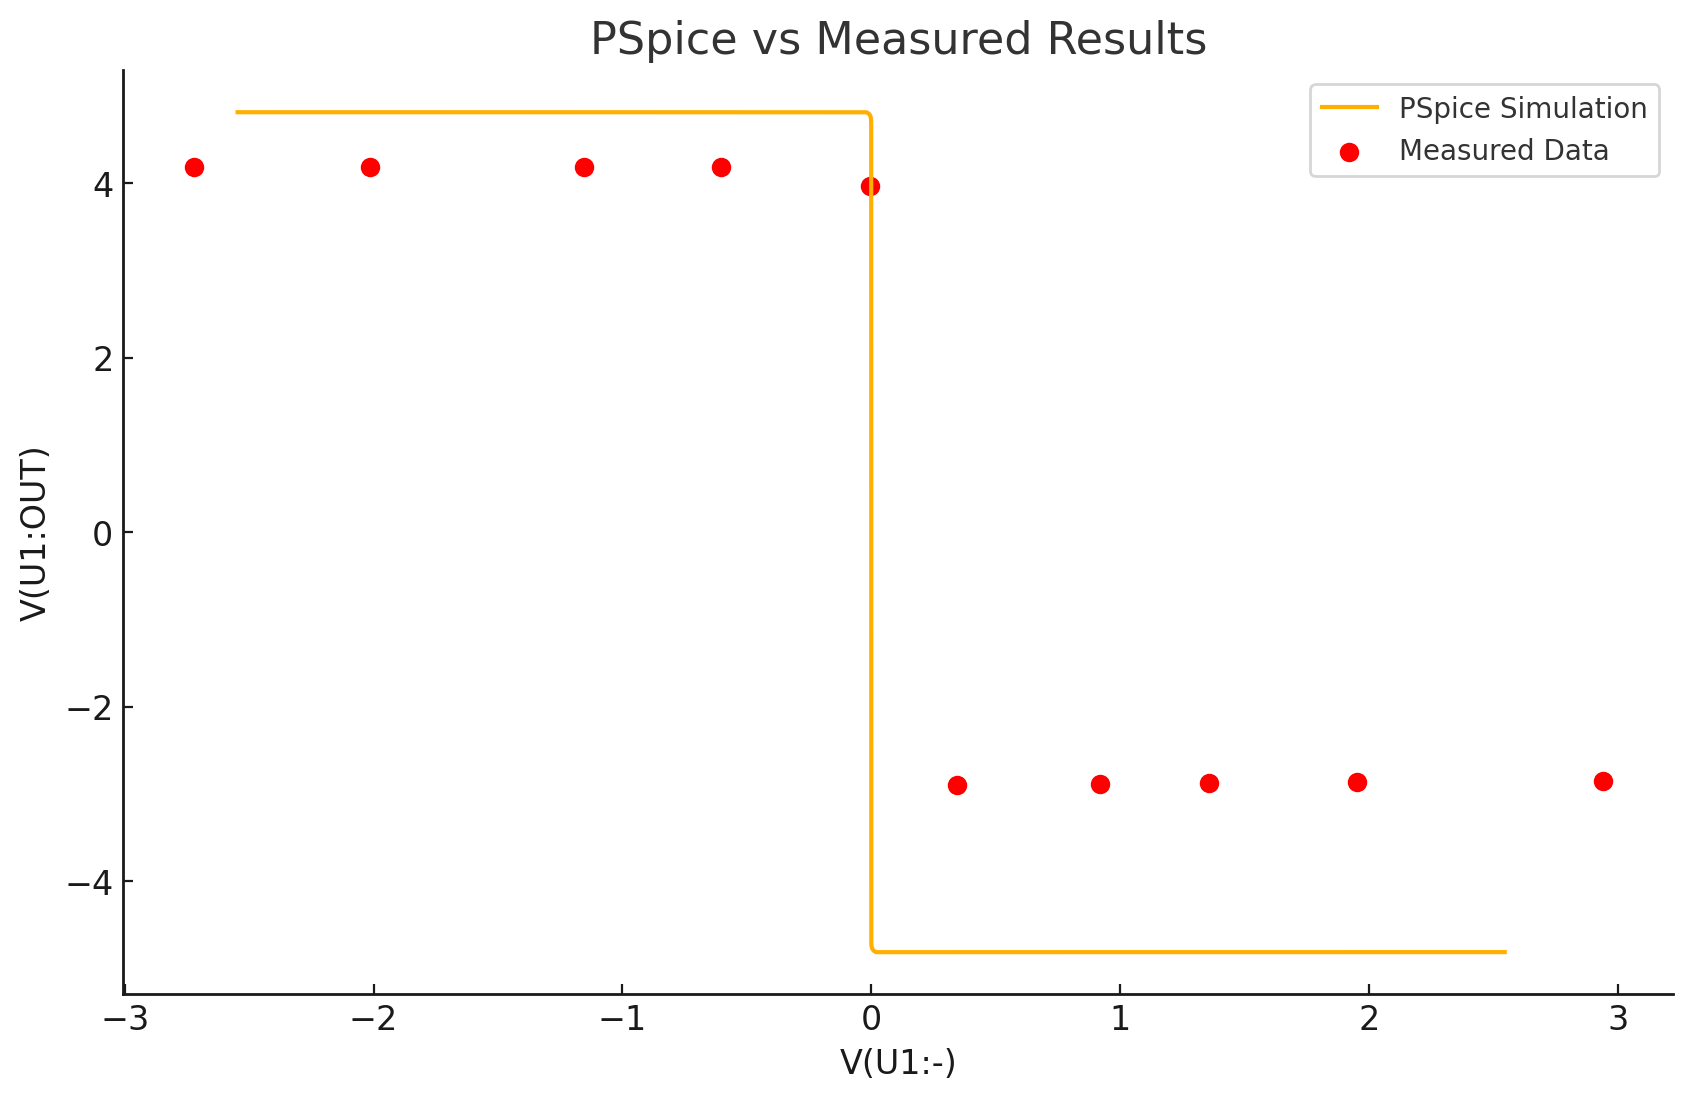
\includegraphics[width=12cm]{03_pspice}
	\caption{Simulated and Measured Characteristics}
	\label{fig:03_pspice}
\end{figure}

Nonetheless, the output voltage during experimentation verified the linear
operation of the operational amplifier and showed how it can be used in a
potential circuit design.

\section{Conclusion}
Through this series of experiments, we explored the fundamental operational
amplifier configurations and their respective behaviors. The feedbackless
amplifier demonstrated the rapid saturation effect, while the comparator circuit
highlighted the utility of reference voltage for decision-making applications.

The night light circuit effectively illustrated the nonlinear response of a
photoresistor, validating its use in light-sensitive applications. Finally, the
inverting amplifier circuit provided a controlled amplification region, proving
the necessity of feedback in maintaining operational stability.

Building and modeling the circuit in Cadence Allegro PSpice allowed for further
enrichment in utilizing the tool to simulate DC circuits and measure ideal
response curves. Comparing this circuit to the one built in the lab offered
insight and explanation to the behavior seen in the recording data.

To summarize, this was an excellent opportunity to learn about utilizing the
operational amplifier IC and lays good groundwork for experimentation to come.
\end{document}
% vim: set ft=tex tw=80 ts=2 sts=2 sw=2 noet spell:
